\documentclass[12pt,journal,compsoc]{IEEEtran}
\usepackage{graphicx}
\DeclareGraphicsExtensions{.pdf,.png,.jpg}
\begin{document}

\title{
	\huge ORIGIN AUTHENTICATION ON QR CODES \\
    \Large Computer Engineering Department, METU}


\author{\normalsize Ozge~Lule(1881366),~Esref~Ozturk(1881762)}


\IEEEtitleabstractindextext{%
\begin{abstract}

During recent years QR codes started to be used in many areas including posters, business and personal cards and mobile application links. However, it brings a danger with itself, that is no one can be sure if qr code is generated  by who. This report is intented  to make a solution to this problem with origin authentication extension to QR codes.

\end{abstract}


\begin{IEEEkeywords}

 QR Codes, Data-Origin authentication, Signature

\end{IEEEkeywords}}


% make the title area
\maketitle

\IEEEdisplaynontitleabstractindextext

\IEEEpeerreviewmaketitle



\section{Introduction}


\IEEEPARstart{Q}{R} code or Quick Response code was originally designed for industrial applications, and has quickly gained popularity in the advertising industry.

With the increasing use of smartphones, QR codes are becoming popular. Smartphone camera can easily read QR codes. Due to fast readability, it is now widely accepted. The use of QR codes is increasing but most users are unaware of the security risks.


Much of these security risks are because the origin of the QR codes are not known. In this article, we aim to show some of the security risks related and come up with a solution which extends QR codes to have data origin authentication.


\subsection{QR Code}
QR code (abbreviated from Quick Response Code) is the trademark for a type of matrix barcode (or two-dimensional barcode) first designed for the automotive industry in Japan. A barcode is a machine-readable optical label that contains information about the item to which it is attached. A QR code uses four standardized encoding modes (numeric, alphanumeric, byte/binary, and kanji) to efficiently store data; extensions may also be used.


\subsubsection{Design}

Unlike the older, one-dimensional barcodes that were designed to be mechanically scanned by a narrow beam of light, a QR code is detected by a 2-dimensional digital image sensor and then digitally analyzed by a programmed processor. The processor locates the three distinctive squares at the corners of the QR code image, using a smaller square (or multiple squares) near the fourth corner to normalize the image for size, orientation, and angle of viewing. The small dots throughout the QR code are then converted to binary numbers and validated with an error-correcting algorithm.

\begin{center}
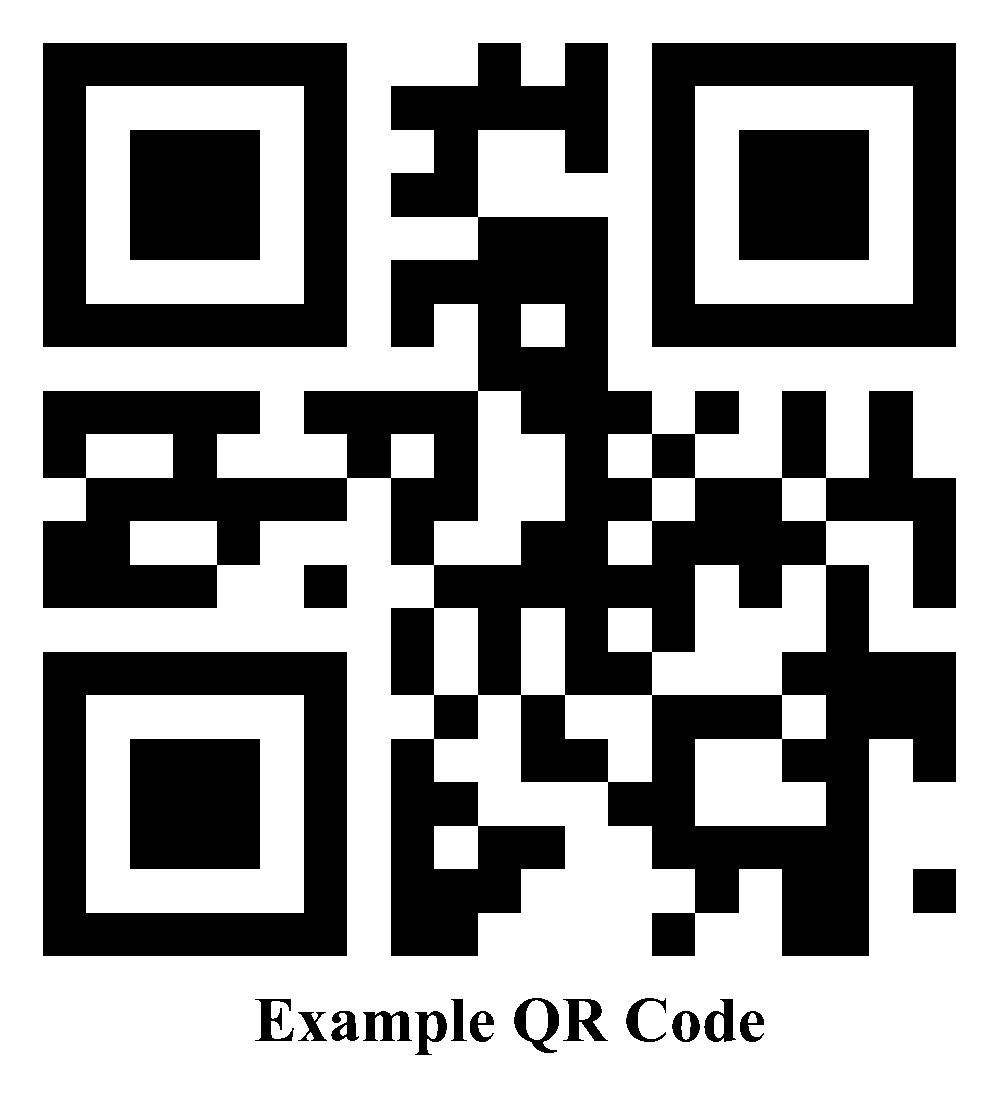
\includegraphics[scale=0.2]{qrcode}
\end{center}


\subsubsection{Uses}

QR codes have become common in consumer advertising. Typically, a smartphone is used as a QR code scanner, displaying the code and converting it to some useful form (such as a standard URL for a website, thereby obviating the need for a user to type it into a web browser). QR code has become a focus of advertising strategy, since it provides a way to access a brand's website more quickly than by manually entering a URL. Usage areas include \textbf{Mobile operating systems, URLS, Code payments, Website logins}.

\subsubsection{Security Risks}

There are various security risks involved with the qr codes.

\textbf{Phishing}


Phishing is the main issue with the QR codes. Attackers send a fake web login page which pretends to be the original login page of the website it’s claiming to be. When an innocent user use this fake page to login, his/her login information is sent to the attacker. And now, his/her password is in the hands of the attacker.



\textbf{Malicious software distribution}

Scammers generally use malicious websites to distribute malware via drive by download attack. Drive by download attacks are attacks in which a website forcefully downloads software in your device when you visit the website. QR codes can be used to point malicious websites. Since QR codes cannot be read, it is easier to trick the user. User is only seeing the reader opening a seemingly harmless web page. In Russia, a malicious QR code on scanning sent SMS to premium numbers costing \$6 USD per SMS.

\textbf{Linking to harmful websites}

Linking to dangerous websites with browser exploits can do a lot harm to user because browser exploits can enable microphone/camera access, send emails or join a botnet to perform a DDOS attack on any legit website.

\subsection{Data origin authentication}

Data origin authentication provides for the corroboration of the source
of a data unit. In a connectionless transfer, it provides assurance that
the source of received data is as claimed.


\section{ORIGIN AUTHENTICATION ON QR CODES}

To achieve origin authentication, qr code should include additional information about the origin that generates it. Also users should be able to check if it is really generated by that origin.

We propose to achieve in 3 steps: 


\subsection{Key Generation}

Firstly, origins should generate a pair of keys, one private and one public. Public key and origin identifier will be put to a public database which maps origin identifier to it's public key. Private key will be kept private by origin.


\begin{center}
\includegraphics[scale=0.6]{KeyGeneration}
\end{center}

\subsection{Encoding}

Once an origin generated keys, it will be able to generate QR codes. Message will be hashed, then encrypted, it other words signed, with the private key of the origin. Afterwards message, signature and origin identifier will be concatenated and it will be used to generate QR code.

\begin{center}
\includegraphics[scale=0.6]{Encoding}
\end{center}


\subsection{Decoding}

QR code will be read and by using origin identifier, public key will be obtained from publicly available directory. Using public key, signature will be decrypted and will be compared to the hash of message. If they are not equal message will be discarded. 


\begin{center}
\includegraphics[scale=0.6]{Decoding}
\end{center}


\begin{thebibliography}{1}

\bibitem{btc}"QR Code features". Denso-Wave. Archived from the original on 2012-09-15. Retrieved 3 October 2011. \\

\bibitem{btc}"QR Code Essentials". Denso ADC. 2011. Retrieved 12 March 2013. \\

\bibitem{btc} \url{http://resources.infosecinstitute.com/security-attacks-via-malicious-qr-codes/ } \\

\bibitem{btc} \url{http://usa.kaspersky.com/about-us/press-center/press-blog/malicious-qr-codes-attack-methods-techniques-infographic} \\

\bibitem{btc} \url{https://en.wikipedia.org/wiki/QR\underline{ }code} \\

\bibitem{btc} \url{http://www.qrcode.com/} \\

\bibitem{btc} \url{https://en.wikiversity.org/wiki/Reed-Solomon\underline{ }codes\_ for\_ coders}


\end{thebibliography}


\end{document}

